\section{Robustness Tests}
\label{sec:c4_robust}

\begin{figure}
\centering
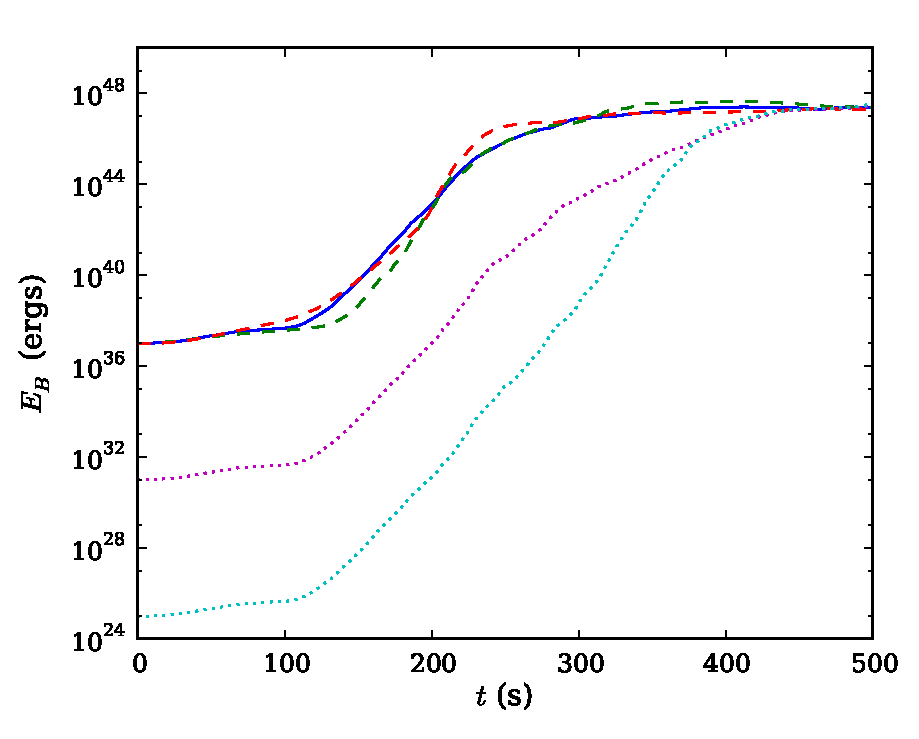
\includegraphics[angle=0,width=0.7\columnwidth]{chapter4_zhu+15/figures/bcomp.pdf}
\caption{Total magnetic energy \EB\ over time for the fiducial (solid blue; $m_\mathrm{cell} \approx 1\times10^{-6}$ \Msun, equatorial surface field strength $10^3$ G) simulation and the robustness tests.  Dashed lines represent low (green; $m_\mathrm{cell} \approx 5\times10^{-6}$ \Msun) and high resolution (red; $m_\mathrm{cell} \approx 2\times10^{-7}$ \Msun) simulations.  Dotted lines represent $1$ G (magenta) and $10^{-3}$ G (cyan) low initial field simulations.}
\label{fig:c4_bcomp}
\end{figure}

\subsection{Resolution Test}
\label{ssec:c4_restest}

To check that our results are not resolution-limited, we performed simulations, otherwise identical to the fiducial one in Sec. \ref{sec:c4_results}, with lower and higher mass resolutions of $m_\mathrm{cell} \approx 5\times10^{-6}$ \Msun\ and $m_\mathrm{cell} \approx 2\times10^{-7}$ \Msun, respectively.  Fig. \ref{fig:c4_bcomp} compares the \EB\ evolution between these simulations (dashed lines) and the fiducial one (solid).

The three runs are qualitatively identical.  Donor disruption and the start of exponential field growth occurs $\sim0.75$ orbital periods earlier at low resolution, and $\sim0.5$ periods later at high, because the outer layers of the WDs are better captured and the differences in hydrostatic equilibrium between \arepo\ and \gasoline\ are less pronounced at higher resolution.  Exponential growth rates are similar between the runs - the \EB\ $e$-folding time is $\tau = 4.9$ s for the low resolution run, faster than $\tau = 6.4$ s for the fiducial.  At high resolution, the growth curve appears to be separated into two phases, with $\tau = 7.8$ s before coalescence, and $\tau = 3.9$ s during it.  The total magnetic energy at the end of exponential growth is also similar - at 400 s, \EB\ is $\sim4\times10^{47}$ ergs in the low resolution run and $\sim1.5\times10^{47}$ ergs in the high, compared to $\sim2\times10^{47}$ ergs at the fiducial resolution.  The fiducial and high resolution runs also qualitatively have very similar magnetic field structures by 400 s.  Our fiducial resolution of $1\times10^{-6}$ \Msun\ therefore appears sufficient for qualitatively capturing the growth and final field configuration of the merger.

In their MHD disk galaxy simulations, \cite{pakms13} find faster field growth and higher field strength at saturation in their lowest resolution run, which they attribute to larger divergence errors at lower resolution.  We perform a similar test, and also see a trend of decreasing divergence error (and more accurate magnetic evolution) at higher resolution, though the errors of all our simulations are at least a factor of two smaller than any reported in \cite{pakms13}.  The errors are highly localized in space and trace steep magnetic gradients, suggesting they contribute only to small-scale variations in the magnetic field.

%In their MHD disk galaxy simulations, \cite{pakms13} find faster field growth and higher field strength at saturation in their lowest resolution run, which they attribute to larger divergence errors at lower resolution.  Performing a similar test, we find the time-averaged \divBrat\ (\divBratnorm) to be $-9.6\times10^{-4}$ ($1.9\times10^{-1}$) for the low resolution, $2.0\times10^{-4}$ ($1.4\times10^{-1}$) for the fiducial, and $7.7\times10^{-5}$ ($1.0\times10^{-1}$) for the high resolution run.  As expected, we see a trend of decreasing divergence error (and more accurate magnetic evolution) at higher resolution, but we note that the errors of all our simulations are at least a factor of two smaller than any reported in \cite{pakms13}.  The errors are highly localized in space and trace steep magnetic gradients, suggesting they contribute only to small-scale variations in the magnetic field.

\subsection{Changing the Seed Field Strength}
\label{ssec:c4_seed}

To understand the dependence of our results on the initial seed field, we ran two additional simulations in which we decreased the strength of the seed field by $3$ and $6$ orders of magnitude leading to an initial equatorial surface field of $1$ G (central field $\sim2\times10^{4}$ G), and $10^{-3}$ G ($\sim20$ G), respectively.  Fig. \ref{fig:c4_bcomp} shows their \EB\ evolution (dotted lines).  We find the growth curves to be homologous between both low initial field runs and the fiducial one -- differing only by the ratios of seed \EB\ -- up to $\sim200$ s, with the $e$-folding time for exponential amplification approximately $6.5$ s for all three runs.  By $\sim250$ s, the field in the fiducial simulation begins to plateau, while amplification (of initially weaker fields) continues for several hundred more seconds in the low initial field runs.  For both runs, \EB\ plateaus at $\sim3\times10^{47}$ ergs, comparable to the fiducial $\sim2\times10^{47}$ ergs.  Because the fields in the low initial field runs remain dynamically irrelevant for longer, however, their structures differ from that of the fiducial run and resemble more the crescent in Fig. \ref{fig:c4_snapshots}, row 4.  The disk field does not saturate in any simulation -- its strength is proportional to the strength of the seed field, and is thus much weaker in the low initial field runs.  Our tests thus suggest that the exponential growth, growth timescale and plateau \EB\ are robust to changes in initial field strength, while the remnant field configuration is more sensitive to the choice of seed field.

\section{Discussion}
\label{sec:c4_discussion}

We have shown that the merger of a 0.625 - 0.65 \Msun\ CO WD binary produces a strong, $>10^{10}$ G magnetic field with a complex structure that winds through the remnant core and into the inner disk.  Similar to previous simulations of binary NS mergers, the strong field is generated by dynamo action within Kelvin-Helmholtz vortices formed during the coalescence of the two WDs.  Since these vortices are ubiquitous in WD mergers, strong magnetic fields are a likely feature of all merger remnants.  The degree to which a field permeates the remnant core depends on how thoroughly the donor and accretor mix during coalescence, which itself is sensitive to initial conditions such as the degree of synchronization between the WDs, or how accurately their tidal bulges and early mass transfer are captured \citep{dan+11, dan+14}.  A parameter space study of magnetized mergers is needed to investigate the range of possible remnant field configurations.

%The highest-resolution NS merger simulations resolve their stars with $\sim100^3$ grid cells, which is approximately the same resolution we use, and a factor of $10^3$ too small to reach the spatial resolution of local vortex simulations.

We note that NS mergers simulated in Eulerian grid codes generally show \EB\ growing by only a factor of $\sim10^2-10^3$ during coalescence, compared to the $\sim10^9$ we see, despite these simulations having resolutions comparable or superior to our low resolution \arepo\ run.  This weaker growth is also inconsistent with the amplification to local kinetic equipartition seen in small-scale simulations \citep{oberam10, zrakm13}, and is attributed to insufficient resolution in the NS merger simulations (\citealt{kiuc+14,giac+15}, though see \citealt{dionar15}).  \cite{giac+15} incorporated a subgrid magnetic amplification model, calibrated using \cite{zrakm13}s results, into their Eulerian NS merger simulation, and found \EB\ amplification by a factor of $\sim10^{10}$ over a single dynamical time.\footnote{\cite{pricr06}s SPH simulations also show strong amplification; while runs using their Euler potential MHD method suffer exaggerated field growth from improper boundary conditions, their $\boldsymbol{B}$-based runs show similar results \citep{pric12}.}  This suggests \arepo\ may be better able to resolve small-scale velocity structures than an Eulerian code at comparable resolution, or better able to couple these structures to magnetic growth.  Further work is needed to understand the magnetic field growth in detail.

The density profile of the remnant remains non-axisymmetric for hundreds of seconds after coalescence.  As a result, the core continues to evolve dynamically, and by 400 s has begun to launch a pair of spiral waves into the surrounding medium (see the density panel of Fig. \ref{fig:c4_remnant}), which transport angular momentum on a timescale rivalling that for magnetic shear.  While \cite{kash+15} report a similar spiral instability in their Eulerian remnant evolution simulation, SPH simulations like those of \citeal{zhu+13} rapidly achieve axisymmetry after coalescence and do not form spiral waves.  As noted earlier, this difference between \arepo\ and SPH simulations is a product of the differences between their hydrodynamic schemes.  Further study is needed to understand these differences and their consequences for remnant evolution \Zhuprep.

%While \cite{schw+12} use an $\alpha$-viscosity to emulate magnetic viscosity

The post-merger evolution of the remnant has been followed to $\sim3\times10^4$ s with axisymmetric cylindrical (two-dimensional) Eulerian grid simulations \citep{schw+12,ji+13}.  As described earlier, \cite{ji+13}s MHD simulation of a 0.6 - 0.6 \Msun\ remnant shows the development of a strong magnetic field due to MRI.  The subsequent heating and angular momentum transport due to the fields pushes core temperatures to ignition, supporting the possibility of a nuclear runaway within sub-\Mch\ remnants.  Their results are, however, likely sensitive both to their initial hydrodynamic conditions -- which may have artificially high core temperatures -- and their chosen seed magnetic field, a pure poloidal one to optimize the onset of MRI.  Our much stronger poloidal-toroidal field could substantially change post-merger evolution.  Moreover, the persistence of a non-axisymmetric remnant core will lead to evolution that clearly cannot be captured in a axisymmetric cylindrical grid.  We therefore stress the need to perform high-resolution three-dimensional simulations of post-merger evolution to determine the final fate of the remnant.

%Schwab et al. doesn't make any mention of a jet, though in our old 2D PME simulations we did find one with only an alpha viscosity installed (those sims aren't to be trusted though).  Their outflow is also limited to < 10^-5 Msun.

There are a number of potentially observable consequences of the magnetic fields produced by the merger.  \cite{ji+13} note the creation of a magnetized corona and biconal jet in their simulations, which act in concert to cause an outflow of material near the remnant's poles.  This outflow eventually unbinds $\sim10^{-3}$ \Msun\ of material, and \cite{belo14} estimates it should lead to an optical transient with a duration of $\sim1$ day and peak $L \sim10^{8}$ \Lsun, which should be detectable by optical surveys.

If a remnant later experiences a nuclear runaway and explodes as a SN Ia, its magnetic field will increase the late-time emission by trapping positrons (produced by $^{56}$Co $\beta^+$ decay) that would otherwise escape the ejecta.  The trapping efficiency depends on the strength and configuration of the remnant magnetic field, with a locally entangled $\sim10^{11}$ G field -- similar to our findings -- well able to trap positrons past 1000 days \citep{ruizs98}.  This is in line with observed late-time SN Ia light curves (most recently \citealt{kerz+14}).

Those remnants that do not explode will retain strong fields when they reach quiescence, and populate the high-mass tail of the distribution of isolated high-field magnetic WDs \citep{garc+12,kule+13,wicktf14,brig+15}.  Since these remnants will have temperatures high enough to fuse any remaining hydrogen and helium they possess, their properties might eventually be akin to the recently discovered hot DQ WDs (e.g. \citealt{dufo+13}).  These WDs have carbon-dominated atmospheres and $T_\mrm{eff} \approx 2\times10^4$ K, are often strongly magnetized ($\sim1$ MG) and sometimes have monoperiodic photometric variability (possibly due to rapid rotation).  Their origins remain unclear \citep{alth+09, lawr+13, will+13}.  Dunlap \& Clemens (in press) recently found that, if most known hot DQs are massive ($M \gtrsim 0.95\Msun$), their population's velocity dispersion corresponds to a kinematic age much older than what would be inferred from their temperatures, suggesting that at least some hot DQs are WD-WD merger remnants.  If so, their observed properties would constrain merger and remnant evolutionary models, and double-degenerate channels for SNe Ia.

\vspace{5mm}

We thank Christopher Thompson, Christopher Matzner, Volker Springel, Bart Dunlap, Yuri Levin, Henk Spruit, Ue-Li Pen and Stephen Ro for their insights into magnetohydrodynamics and simulations.  This work utilized the SciNet HPC Consortium's GPC supercomputer \citep{loke+10}.  C.Z. acknowledges support from the Natural Sciences and Engineering Research Council (NSERC) Vanier Canada Graduate Scholarship.  R.P. acknowledges support by the European Research Council under ERC-StG grant EXAGAL-308037 and by the Klaus Tschira Foundation.  P.C. is supported by the NASA ATP program through NASA grant NNX13AH43G, and NSF grant AST-1255469.  
